\documentclass[10pt,a4paper]{article}
\usepackage[slovak]{babel}
\usepackage[utf8]{inputenc}
\usepackage{amsmath}
\usepackage{amsfonts}
\usepackage{amssymb}
\usepackage[unicode]{hyperref}
\usepackage{graphicx}

\textwidth 6.5in
\oddsidemargin 0.0in
\evensidemargin 0.0in

\title{Poznámky z Úvodu do databázových systémov - materiál na štátnice}
\date{16.06.2012}
\author{Peter Csiba, petherz@gmail.com, \url{https://github.com/Petrzlen/fmfi-poznamky}} 

\begin{document}
\maketitle
\tableofcontents

\clearpage

%%%%%%%%%%%%%%%%%%%%%%%%%%%%%%%%%%%%%%%%%%%%%%%%%%%%%%%%%%%%%%%%%%%%%%%%%%%%%%%%
%%%%%%%%%%%%%%%%%%%%%%%%%%%%%%%%%%%%%%%%%%%%%%%%%%%%%%%%%%%%%%%%%%%%%%%%%%%%%%%%
\section*{Úvod}   

Text je poznámkami k oficiálnym \href{http://new.dcs.fmph.uniba.sk/index.php/Studium/Bakalarske/StatneSkusky}{štátnicovým otázkam} a boli spísané počas učenia sa na ne.
Poznámky sa nesnažia ísť do hĺbky (na to je H.Garcia-Molina, Ullman a Wikipédia).
Naopak, snažia sa priniesť intuitívnu predstavu o algoritmoch a pojmoch a dávať ich do súvisu.

Poznámky sú organizované podľa štátnicových otázok, snažia sa minimalizovať omáčku a nevysvetlujú a neuvádzajú do problematiky. Text je určený čitateľom, ktorý sa už s hlavnými pojmami stretli.
Autor považuje všetky otázky za rovnako dôležité a odporúča v prípade slabšieho pochopenia samostatne vypracovať niektoré staré \href{http://www.dcs.fmph.uniba.sk/~plachetk/TEACHING/DB2011/index.html}{písomky}.

Autor absolvoval základný test predmetu Úvodu do databázových systémov s hodnotením A, a má základné skúsenosti s administráciou a návrhom databáz. Napriek tomu autor \underline{neručí za kvalitu a úplnosť textu} a čitateľov \underline{aj} preto autor \underline{prudko odporúča pozrieť si aj iné zdroje}. Uvedieme citát\footnote{Dr. Tomas Plachetka, Uvod do databazovych systemov 2011/2012 Zima} ''Tieto slajdy sú sprievodcom pri prednáške, nie sú myslené ako náhrada
prednášky či nebodaj knihy. K príprave na skúšku nestačí len prečítať slajdy'', niečo také sú aj tieto poznámky.  

Nakoniec poznamenajme, že autor sa snažil písať pravdu a len pravdu, keďže jeho odpoveď na záverečných skúškach vychádza z tototo materiálu.
Ak čitateľ chce prispieť ku kvalite textu, nech autorovi napíše a ten mu udelí prístup do repozitára.

P.S. Autor zistil, že názvoslovie pijan, ľúbi, krčma, alkohol použil už napríklad \href{http://csip.sk/uploads/ullman.pdf}{Ullman}.

%%%%%%%%%%%%%%%%%%%%%%%%%%%%%%%%%%%%%%%%%%%%%%%%%%%%%%%%%%%%%%%%%%%%%%%%%%%%%%%%
%%%%%%%%%%%%%%%%%%%%%%%%%%%%%%%%%%%%%%%%%%%%%%%%%%%%%%%%%%%%%%%%%%%%%%%%%%%%%%%%
\section*{Úvod a motivácia databáz}
\paragraph{Účel.}
\begin{itemize}
\item Zobrazenie vybranej časti reality v počítačí.
\item Uchovávanie informácií v konzistentnom stave a ich pridávanie.
\item Poskytovanie informácií (dotazy, reporty - periodické správy). 
\item Ochrana informácií pred zničením a neoprávneným prístupom. 
\end{itemize}

\paragraph{Charakteristiky DBMS (Database Management System).}
\begin{itemize}
\item Dáta majú štruktúru, ktorá sa zriedka mení, objem dát je veľký.
\item Dáta nie sú uložené na užívateľovom počítači, pre prístup k dátam sa využíva počítačová sieť (klient-server).
\item Dotazy sú zložité.
\item Množstvo užívateľov pristupuje k dátam súčasne.
\item Vyžaduje sa vysoká priepustnosť.
\item Vyžaduje sa vysoká odolnosť voči poruchám.
\item Vyžaduje sa vysoký stupeň bezpečnosti.
\item Prístup koncových užívateľov k dátam musí byť jednoduchý(API, GUI).
\end{itemize}

\paragraph{Porovnanie dotazov v dátových modeloch.}
Vo všeobecnosti sa snažíme zbaviť všeobecných kvatifikátorov pomocou pravidla $\forall P \rightarrow \neg \exists \neg P$.

Máme tabuľky: 
\begin{itemize}
\item studenti(Student, Skupina)
\item rozvrh\_skupiny(Skupina, Miestnost, Cas)
\item rozvrh\_ucitelia(Ucitel, Skupina)
\end{itemize}

\begin{itemize}
\item \emph{Hovorovo.} Treba nájsť (všetky) štvorice [Student, Miestnost, Cas, Ucitel]
také, že ten učiteľ učí toho študenta v tej miestnosti a tom čase. 
\item \emph{Predikátový kalkul.}

\{[Student, Miestnost, Cas, Ucitel]: $\exists$ Skupina (Student, Skupina) $\wedge$ rozvrh\_skupiny(Skupina, Miestnost, Cas) $\wedge$ rozvrh\_ucitelia(Ucitel, Skupina)\}
\item \emph{Relačná algebra.}
$$
\Pi_{student, miestnost, cas, ucitel}(studenti \Join rozvrh_skupiny \Join rozvrh_ucitelia)
$$
\item \emph{Datalog (Prolog).}
\begin{verbatim}
rozvrh_studenti(Student, Miestnost, Cas, Ucitel) <--
\begin{verbatim}
  studenti(Student, Skupina),
  rozvrh_skupiny(Skupina, Miestnost, Cas),
  rozvrh_ucitelia(Učitel, Skupina).

? rozvrh_studenti(S, M, C, U)
\end{verbatim} 

\item \emph{SQL.}
\begin{verbatim}
SELECT S.student, RK.miestnost, RK.cas, RU.ucitel
FROM studenti S, rozvrh_skupiny RK, rozvrh_ucitelia RU
WHERE S.skupina=RK.skupina AND S.skupina=RU.skupina
\end{verbatim}

\end{itemize}

%%%%%%%%%%%%%%%%%%%%%%%%%%%%%%%%%%%%%%%%%%%%%%%%%%%%%%%%%%%%%%%%%%%%%%%%%%%%%%%%
%%%%%%%%%%%%%%%%%%%%%%%%%%%%%%%%%%%%%%%%%%%%%%%%%%%%%%%%%%%%%%%%%%%%%%%%%%%%%%%%
%TODO vynechava stranu, (asi) lebo article a section* a section
\section{Dátové modely} 
\href{http://en.wikipedia.org/wiki/Database_model}{Pozri Wikipédiu.}

\paragraph{Používané dátové modely.}
\begin{itemize}
\item Entitno-relačný. Pozri \ref{entity_relationship}. 
\item Relačný. Pozri \ref{relacny_kalkul} a \ref{relacna_algebra}. 
\item Navigačný (XML). Stromová štruktúra, dotazovací jazyk XPath a XQuery. 
\item Objektový. Niečo ako objekty v programovaní. Objekty okrem zapuzdrenia dát špecifikujú prístup k nim a k ich vzťahom, je možné s nimi programaticky narábať. Napríklad DOM (Document Object Model). 
\end{itemize}


%%%%%%%%%%%%%%%%%%%%%%%%%%%%%%%%%%%%%%%
\subsection{Trojschémová architektúra (ANSI sparc)}

\paragraph{Úrovne.}
\begin{itemize}
\item Konceptuálna úroveň (všeobecná databázová schéma). 
\item Interná úroveň (špecifikácia polí, kľúčov, indexov, ...).
\item Fyzická úroveň. Algoritmy a dátové štruktúry, využtie diskového priestoru. Pozri \ref{fyzicka_organizacia}.
\end{itemize}

\begin{center}
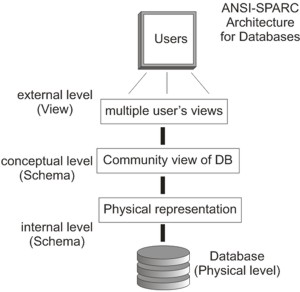
\includegraphics[scale=0.5]{db_ansi_sparc.jpg}
\end{center} 

\paragraph{Vlastnosti.}
\begin{itemize}
\item Nezávislý pohľad užívateľov. Každý môže použiť svoj dotazovací jazyk. 
\item Užívateľ nevidí fyzickú organizáciu dát. Tá sa môže zmeniť, bez toho, aby to užívateľ postrehol. 
\end{itemize}

%%%%%%%%%%%%%%%%%%%%%%%%%%%%%%%%%%%%%%%
\subsection{Entitno-relačný model}
\label{entity_relationship}

Máme entity (tabuľky, polia, ...) a vzťahy medzi nimi. 
\paragraph{Typy vzťahov.}
\begin{itemize}
\item One-to-one (1-1). Napríklad hlava a telo. 
\item One-to-many (1-n). Napríklad vozidlo a kolesá. 
\item Many-to-many (n-m). Napríklad kupujúci a produkt (táto dvojica nemusí byť unikátna).
\end{itemize}

\begin{center}
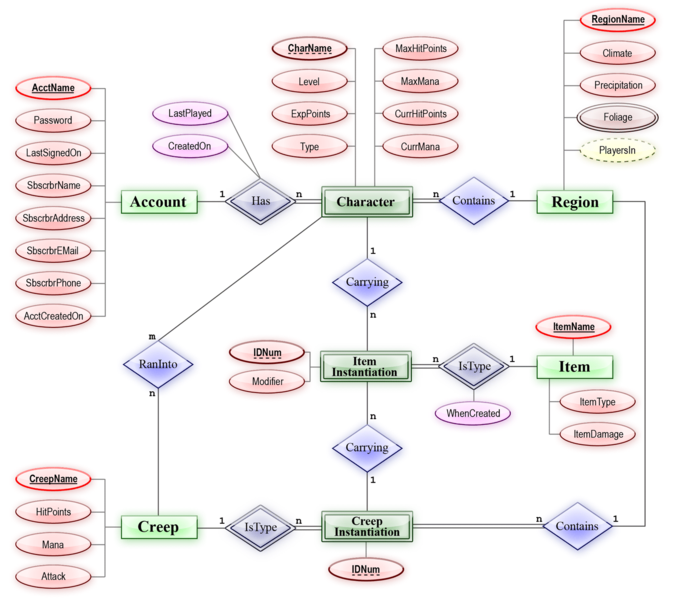
\includegraphics[scale=0.5]{db_entity_relationship.png}
\end{center} 

%%%%%%%%%%%%%%%%%%%%%%%%%%%%%%%%%%%%%%%
\subsection{Relačný model, relačná algebra}
Pozri \ref{relacny_kalkul} a \ref{relacna_algebra}. 

%%%%%%%%%%%%%%%%%%%%%%%%%%%%%%%%%%%%%%%
\subsection{Negácia a rekurzia v relačnej algebre}
Pozri \ref{relacna_algebra}. 

%%%%%%%%%%%%%%%%%%%%%%%%%%%%%%%%%%%%%%%
\subsection{Súvis relačnej algebry s inými dotazovacími jazykmi}
Pozri \ref{relacna_algebra_suvis}.
    
%%%%%%%%%%%%%%%%%%%%%%%%%%%%%%%%%%%%%%%%%%%%%%%%%%%%%%%%%%%%%%%%%%%%%%%%%%%%%%%%
%%%%%%%%%%%%%%%%%%%%%%%%%%%%%%%%%%%%%%%%%%%%%%%%%%%%%%%%%%%%%%%%%%%%%%%%%%%%%%%%
\section{Relačný kalkul} 
\label{relacny_kalkul}

Deklaruje výroky, ktoré ohraničujú výsledok dotazu. 
\paragraph{Použité pojmy.}
Je odporúčané vedieť matematickú logiku. 

\begin{itemize}
\item $n$-árna relácia (konečná, nekonečná). Usporiadané $n$-tice. Karteziánsky súčin. 
\item Atribúty - zložky $n$-tíc. Domény (typy atribútov) - množiny karteziánskeho súčinu. 
\item Predikát $P$ prislúchajúci relácií $R$- zobrazenie $R_P : R \mapsto$ \{true, false\}, pričom $R_P(A) = true \leftrightarrow A \in R$, kde $A$ je usporiadaná $n$-tica. V praxi medzi tým nerozlišujeme. 
\end{itemize}

\paragraph{Dotaz.}
Dotazy v relačnom kalkule sú logické formuly predikátovej logiky prvého rádu.
Formula by nemala mať voľné premenné. Výsledkom sú prvky relácie, ktoré spĺňajú formulu. 

%%%%%%%%%%%%%%%%%%%%%%%%%%%%%%%%%%%%%%%
\subsection{Predikátová interpretácia relačnej algebry}
??? Asi ide o prepis symbolov relačnej algebry do predikátovej logiky. 
%TODO 

%%%%%%%%%%%%%%%%%%%%%%%%%%%%%%%%%%%%%%%
\subsection{Negácia, doménovo nezávislé a bezpečné formuly}

\paragraph{Príklad dotazov.}
\begin{enumerate}
\item prvocisla1: $\{Z : (\forall X) (\forall Y) (krat(X,Y,Z) \rightarrow X = 1 \wedge Y = 1)\}$.
\item zlozene\_cisla: $\{Z : (\exists X) (\exists Y) (krat(X,Y,Z) \wedge X \neq 1 \wedge Y \neq 1)\}$.
\item prvocisla2: $\{Z : (\exists X) (\exists Y) (krat(X,Y,Z) \wedge Z \notin zlozene\_cisla) \}$.
\item prvocisla3: $\{Z : Z \notin zlozene\_cisla\}$.
\end{enumerate}
Tretiu formulu (reláciu, resp. množinu) sme získali dvojitou negáciou prvej a pravidlom $P \rightarrow Q \Leftrightarrow \neg P \vee Q$ (medzi krok je druhá formula). 

Formuly pre prvocisla1 a prvocisla3 sú \emph{nebezpečné}, keďže ich výsledom je napríklad aj ''petrzlen''.
V prvom prípade je implikácia pravdivá (lebo ľavá strana je nepravdivá) a v druhom prípade je to zjavné, keďže ''petrzlen'' nie je zložené číslo. 
Správna je len formula prvocisla2. 

\emph{Množina faktov} (nazývaná aj \emph{extenzionálna databáza (EDB)}) je \underline{konečná} množina, na ktorej je predikát v dotaze pravdivý (to zrejme neplati pre prvocisla1 a prvocisla3, ale platí pre prvocisla2 a zlozene\_cisla).
Neformálne, \emph{bezpečný dotaz} je taký, v ktorom sa každá premenná vyskytuje v aspoň jednom EDB v pozitívnom kontexte. Tj. chceme, aby sa premenná \underline{ne}vyskytovala v negovanej množine faktov (výroku). Napríklad v prvocisla3 je $Z$ v negatívnom kontexte.  

%%%%%%%%%%%%%%%%%%%%%%%%%%%%%%%%%%%%%%%
\subsection{Relačný kalkul (doménový)}

Myslím, že je to popísané v predošlých sekciách.
Pripomeňme, že \emph{domény} sú typy atribútov - množiny karteziánskeho súčinu.


%%%%%%%%%%%%%%%%%%%%%%%%%%%%%%%%%%%%%%%
\subsection{Súvis relačného kalkulu s inými dotazovacími jazykmi}
Základná intuícia. Celkom dobre sa doň prekladá z hovorového a jendoducho sa z neho konštruuje datalog, resp. relačná algebra.
V praxi nie je použiteľný, keďže ide o teoretický model (s potenciálne nekonečnými reláciami). 
    
%TODO 

%%%%%%%%%%%%%%%%%%%%%%%%%%%%%%%%%%%%%%%%%%%%%%%%%%%%%%%%%%%%%%%%%%%%%%%%%%%%%%%%
%%%%%%%%%%%%%%%%%%%%%%%%%%%%%%%%%%%%%%%%%%%%%%%%%%%%%%%%%%%%%%%%%%%%%%%%%%%%%%%%
\section{Datalog} 
\href{http://en.wikipedia.org/wiki/Datalog}{Datalog} je dotazovací jazyk s pravidlami určený pre deduktívne databázy, ktorý je syntakticky podmnožinou Prologu. Je založený na predikátovej logike prvého rádu (neumožňuje kvantifikovať množiny). 

Odporúčame si pozrieť slide-i Plachetku pre ďalšie príklady dotazov.
Ideálne si niektoré úlohy treba vyskúšať v Datalógovom interpretery (tak sa to učí najlepšie).

%%%%%%%%%%%%%%%%%%%%%%%%%%%%%%%%%%%%%%%
\subsection{Syntax a sémantika Datalogových programov}

\paragraph{Syntax.}
Program pozostáva z množiny pravidiel - \emph{implikácií} - \emph{predikátov}, ktoré majú \emph{hlavu} a \emph{telo}\footnote{
Nie pätu. Poznámka autora. 
} (ľavá a pravá strana implikácie, resp. \emph{premisa} a \emph{dôsledok}). 
Napríklad:
\begin{verbatim}
1. krat(1, 1, 1) <-- TRUE.
2. krat(1, 1, 1).
3. zlozene_cislo(Z) <--
  krat(X, Y, Z),
  not X = 1,
  not Y = 1.
4. prvocislo(Z) <--
  krat(X, Y, Z),
  not zlozene_cislo(Z)
5. prvocislo(Z) <--
  krat(_, _, Z),
  not zlozene_cislo(Z)
\end{verbatim} 
Predikáty 1 a 2 a aj predikáty 4 a 5 sú sémanticky ekvivalentné. Premenné na ľavej strane sú kvantifikované $\forall$ a premenné na pravej strane $\exists$. Čiarka medzi atómami má význam AND. Bodka označuje koniec predikátu. \emph{Podcieľmi} nazývame atómy tela rozdelené čiarkami, napríklad 
  \verb|{krat(_, _, Z)}| a \verb|not zlozene_cislo(Z)| sú podcieľmi \verb|prvocislo(Z)|. 
V 5 používame \emph{anonymné premenné} ''\_''. Ich sémentika je rovnaká, ako keby sa použila ľubovoľná nepoužitá premenná. Poznmenajme, že v tele pravidla sú premenné implicitne kvantifikované $\exists$.
  
Alebo (disjunkcia) sa vyjadruje:
\begin{verbatim}
colour(F) <-- F = black
colour(F) <-- F = white
\end{verbatim} 
  
\paragraph{Ďalšie syntaktické pravidlá.}

\begin{itemize}
\item Argumentmi (hláv) predikátov môžu byť len jednoduché atribúty. Nemôžeme \verb|zlozene_cislo(f(f(Z,5)) <-- |. 
\item (Tvrdí Wiki, nie Plachetka). Každá premenná v hlave predikátu sa musí vyskytovať aj v nie negovanom podcieli predikátu (súvisí s bezpečnosťou). 
\end{itemize}

\paragraph{Sémantika.}
Je založená na relačnom kalkule (a matematickej logike). 
Niečo sa spomenulo vyššie, doplňujeme v ďalšej sekcií. 

%%%%%%%%%%%%%%%%%%%%%%%%%%%%%%%%%%%%%%%
\subsection{Súvis s relačným kalkulom}

Napríklad 
\begin{verbatim}
3. zlozene_cislo(Z) <--
  krat(X, Y, Z),
  not X = 1,
  not Y = 1.
\end{verbatim} 
je sémanticky ekvivalentným programom k $$
zlozene\_cisla: \{Z : (\exists X) (\exists Y) (krat(X,Y,Z) \wedge X \neq 1 \wedge Y \neq 1)\}.
$$


Existuje algoritmický predklad medzi týmito dvoma modelmi.
Algoritmus, ktorý prepisuje relačný kalkul do Datalogu pozostáva z nasledujúcich krokov (treba ich vedieť \underline{použiť}):

\begin{enumerate}
\item Premenovanie premenných, lokalizácia kvantifikátorov. Vlastne veta o variantoch z matematickej logiky. 

\item Eliminácia všeobecných kvantifikátorov a implikácií. Použijeme pravidlá $(\forall x)A(x) \leftrightarrow \neg (\exists x) \neg A(x)$ a $(A \rightarrow B) \leftrightarrow (\neg A \vee B)$.

\item Definícia pomocných predikátov. Chceme sa vyhnúť sekvencií $\neg (\exists X) povodny\_predikat(X)$. Definujeme preto pomocné predikáty: 
$$
\begin{array}{l}
\neg novy\_predikat \\
novy\_predikat \leftarrow (\exists X) povodny\_predikat(X).\\
\end{array} 
$$

\item Bezpečnosť pomocných predikátov. Pridáme k premenným ich dómeny:
$$
novy\_predikat \leftarrow domena(X) \wedge (\exists X) povodny\_predikat(X).
$$

\item Prepis do pravidiel Datalogu. Len zmeniť syntax:
\begin{verbatim}
answer <-- not novy_predikat.
novy_predikat <-- povodny_predikat(X).
\end{verbatim}

\end{enumerate}

Poznamenajme, že podobne existuje algoritmus, ktorý prepisuje datalogove dotazy do SQL (tiež treba vedieť použiť). 

%%%%%%%%%%%%%%%%%%%%%%%%%%%%%%%%%%%%%%%
\subsection{Výpočet dotazu na Datalogový program}

Datalog počíta \emph{minimálny model} programu (minimálne relácie, pre ktoré je daný program splnený). Inými slovami, Datalog vracia najmenšiu množinu, pre ktorú sú splnené všetky potrebné predikáty, na ktorých závisí dôsledok (dotaz). Tj. neuvažuje také výsledky, pre ktoré sú predpoklady nesplnené. Napríklad program: 
\begin{verbatim}
colour(black).
colour(white).
? colour(C).
\end{verbatim}
by mohol vrátiť aj ''mrkva'', lebo nič tomu neodporuje.

Minimálny model existuje pre každý \emph{bezpečný program} (ktorý sa definuje prakticky rovnako, ako v relačnom kalkule).

%%%%%%%%%%%%%%%%%%%%%%%%%%%%%%%%%%%%%%%
\subsection{Negácia}

\paragraph{Russelov paradox.}
\begin{verbatim}
man(barber).
man(mayor).
shaves(barber, X) <-- man(X), not shaves(X, X).
? shaves(barber, barber)
\end{verbatim}

Paradox nenastáva, keďže pravidlo je definované ako implikácia. Výsledok nemôže byť FALSE,
lebo by predpoklad bol splnený. Ak je výsledok TRUE, tak \verb|man(X), not shaves(X, X) --> shaves(barber, X)| platí. 

%%%%%%%%%%%%%%%%%%%%%%%%%%%%%%%%%%%%%%%
\subsection{Bezpečnosť Datalogových programov}

\emph{Bezpečný predikát} je taký, ktorého všetky premenné vyskytytujúce sa v hlave, sú viazané v EDB. 

\emph{Bezpečný program} má všetky svoje predikáty bezpečené. 

(Zopakujeme) Minimálny model existuje pre každý bezpečný program (ktorý sa definuje prakticky rovnako, ako v relačnom kalkule).
 
Všeobecne platí, že anonymné premenné v negovaných EDB podcieľoch
nespôsobujú problém s bezpečnosťou.
 
Pán Šturc definujeme slabšie podmienky. 
    
%%%%%%%%%%%%%%%%%%%%%%%%%%%%%%%%%%%%%%%%%%%%%%%%%%%%%%%%%%%%%%%%%%%%%%%%%%%%%%%%
%%%%%%%%%%%%%%%%%%%%%%%%%%%%%%%%%%%%%%%%%%%%%%%%%%%%%%%%%%%%%%%%%%%%%%%%%%%%%%%%
\section{Relačná algebra} 
\label{relacna_algebra}

%%%%%%%%%%%%%%%%%%%%%%%%%%%%%%%%%%%%%%%
\subsection{Operátory relačnej algebry}
%%%%%%%%%%%%%%%%%%%%%%%%%%%%%%%%%%%%%%%
\subsection{Multimnožinová interpretácia relácií}
%%%%%%%%%%%%%%%%%%%%%%%%%%%%%%%%%%%%%%%
\subsection{Grupovanie a agregácia}
%%%%%%%%%%%%%%%%%%%%%%%%%%%%%%%%%%%%%%%
\subsection{Rekurzia, výpočet pevného bodu}
%%%%%%%%%%%%%%%%%%%%%%%%%%%%%%%%%%%%%%%
\subsection{Súvis relačnej algebry s inými dotazovacími jazykmi}
\label{relacna_algebra_suvis}
    
%%%%%%%%%%%%%%%%%%%%%%%%%%%%%%%%%%%%%%%%%%%%%%%%%%%%%%%%%%%%%%%%%%%%%%%%%%%%%%%%
%%%%%%%%%%%%%%%%%%%%%%%%%%%%%%%%%%%%%%%%%%%%%%%%%%%%%%%%%%%%%%%%%%%%%%%%%%%%%%%%
\section{Jazyk SQL} 
%%%%%%%%%%%%%%%%%%%%%%%%%%%%%%%%%%%%%%%
\subsection{Programovanie v SQL (Data Definition Language, Data Manipulation Language)}
%%%%%%%%%%%%%%%%%%%%%%%%%%%%%%%%%%%%%%%
\subsection{Negácia a rekurzia v SQL}
%%%%%%%%%%%%%%%%%%%%%%%%%%%%%%%%%%%%%%%
\subsection{Súvis SQL s inými dotazovacími jazykmi}
    
%%%%%%%%%%%%%%%%%%%%%%%%%%%%%%%%%%%%%%%%%%%%%%%%%%%%%%%%%%%%%%%%%%%%%%%%%%%%%%%%
%%%%%%%%%%%%%%%%%%%%%%%%%%%%%%%%%%%%%%%%%%%%%%%%%%%%%%%%%%%%%%%%%%%%%%%%%%%%%%%%
\section{Teória navrhovania relačných báz dát} 

%%%%%%%%%%%%%%%%%%%%%%%%%%%%%%%%%%%%%%%
\subsection{Funkčné závislosti}
%%%%%%%%%%%%%%%%%%%%
\paragraph{Armstrongove axiómy.} 
%%%%%%%%%%%%%%%%%%%%
\paragraph{Uzáver množiny atribútov.}
%%%%%%%%%%%%%%%%%%%%
\paragraph{uzáver množiny funkčných závislostí.}

%%%%%%%%%%%%%%%%%%%%%%%%%%%%%%%%%%%%%%%
\subsection{Pokrytie a minimálne pokrytie množiny funkčných závislostí}
%%%%%%%%%%%%%%%%%%%%%%%%%%%%%%%%%%%%%%%
\subsection{Nadkľúče a kľúče}
    
%%%%%%%%%%%%%%%%%%%%%%%%%%%%%%%%%%%%%%%%%%%%%%%%%%%%%%%%%%%%%%%%%%%%%%%%%%%%%%%%
%%%%%%%%%%%%%%%%%%%%%%%%%%%%%%%%%%%%%%%%%%%%%%%%%%%%%%%%%%%%%%%%%%%%%%%%%%%%%%%%
\section{Normálne formy} 
%%%%%%%%%%%%%%%%%%%%%%%%%%%%%%%%%%%%%%%
\subsection{3NF, BCNF}
%%%%%%%%%%%%%%%%%%%%%%%%%%%%%%%%%%%%%%%
\subsection{Algoritmy pre dekompozíciu do normálnych foriem}
%%%%%%%%%%%%%%%%%%%%%%%%%%%%%%%%%%%%%%%
\subsection{Bezstratovosť dekompozície}
    
%%%%%%%%%%%%%%%%%%%%%%%%%%%%%%%%%%%%%%%%%%%%%%%%%%%%%%%%%%%%%%%%%%%%%%%%%%%%%%%%
%%%%%%%%%%%%%%%%%%%%%%%%%%%%%%%%%%%%%%%%%%%%%%%%%%%%%%%%%%%%%%%%%%%%%%%%%%%%%%%%
\section{Transakcie} 
%%%%%%%%%%%%%%%%%%%%%%%%%%%%%%%%%%%%%%%
\subsection{Požiadavky na transakčný systém (ACID)}
%%%%%%%%%%%%%%%%%%%%%%%%%%%%%%%%%%%%%%%
\subsection{Architektúra transakčného systému}
%%%%%%%%%%%%%%%%%%%%%%%%%%%%%%%%%%%%%%%
\subsection{Rozvrhy}
%%%%%%%%%%%%%%%%%%%%%%%%%%%%%%%%%%%%%%%
\subsection{Triedy sériovateľnosti a obnoviteľnosti}
    
%%%%%%%%%%%%%%%%%%%%%%%%%%%%%%%%%%%%%%%%%%%%%%%%%%%%%%%%%%%%%%%%%%%%%%%%%%%%%%%%
%%%%%%%%%%%%%%%%%%%%%%%%%%%%%%%%%%%%%%%%%%%%%%%%%%%%%%%%%%%%%%%%%%%%%%%%%%%%%%%%
\section{Implementácia sériovateľnosti a obnoviteľnosti v transakčných systémoch} 
%%%%%%%%%%%%%%%%%%%%%%%%%%%%%%%%%%%%%%%
\subsection{Testy sériovateľnosti}
%%%%%%%%%%%%%%%%%%%%%%%%%%%%%%%%%%%%%%%
\subsection{Algoritmy izolácie, zámky, časové pečiatky, validácia}
%%%%%%%%%%%%%%%%%%%%%%%%%%%%%%%%%%%%%%%
\subsection{Uviaznutie (deadlock) a metódy riešenia uviaznutia}
%%%%%%%%%%%%%%%%%%%%%%%%%%%%%%%%%%%%%%%
\subsection{Algoritmy obnovy, log-file, checkpointing, backup}
    
%%%%%%%%%%%%%%%%%%%%%%%%%%%%%%%%%%%%%%%%%%%%%%%%%%%%%%%%%%%%%%%%%%%%%%%%%%%%%%%%
%%%%%%%%%%%%%%%%%%%%%%%%%%%%%%%%%%%%%%%%%%%%%%%%%%%%%%%%%%%%%%%%%%%%%%%%%%%%%%%%
\section{Fyzická organizácia} 
\label{fyzicka_organizacia}

%%%%%%%%%%%%%%%%%%%%%%%%%%%%%%%%%%%%%%%
\subsection{Dvojúrovňový model pamäti a organizácie dát}
%%%%%%%%%%%%%%%%%%%%%%%%%%%%%%%%%%%%%%%
\subsection{Indexové stromy, hashovanie}
%%%%%%%%%%%%%%%%%%%%%%%%%%%%%%%%%%%%%%%
\subsection{Operátory fyzickej algebry}
%%%%%%%%%%%%%%%%%%%%%%%%%%%%%%%%%%%%%%%
\subsection{Implementácia vybraných fyzických operátorov (merge-sort, nested-loop join)}


%%%%%%%%%%%%%%%%%%%%%%%%%%%%%%%%%%%%%%%%%%%%%%%%%%%%%%%%%%%%%%%%%%%%%%%%%%%%%%%%
%%%%%%%%%%%%%%%%%%%%%%%%%%%%%%%%%%%%%%%%%%%%%%%%%%%%%%%%%%%%%%%%%%%%%%%%%%%%%%%%
\clearpage
\section*{Referencie a odporúčaná literatúra}
\begin{itemize}                                
\item \href{http://www.dcs.fmph.uniba.sk/~plachetk/TEACHING/DB2011/index.html}{Úvodu do databázových systémov - Plachetka}.        
\item \href{http://www.dcs.fmph.uniba.sk/~sturc/databazy/uvod/}{Úvodu do databázových systémov - Šturc} - v niečom detailnejší.        
\item \href{http://infolab.stanford.edu/~widom/cs145/}{Úvodu do databázových systémov - Stanford University} - základ podobný.


\item \href{http://csip.sk/uploads/plachetka\_uvod\_do\_databaz\_2011.pdf}{Plachetkove slide-i}.
\item \href{http://csip.sk/uploads/ullman.pdf}{Ullmanove slide-i}.
\item \href{http://fmfi-uk.hq.sk/Informatika/Uvod\%20Do\%20Databazovych\%20Systemov/prednasky/}{Mandos}.
\item H. Garcia-Molina, J.D. Ullman, J. Widom: Database Systems, The Complete Book, Prentice Hall, 2003
\item R. Elmasri, S.B. Navathe: Fundamentals of Database Systems, Addison-Wesley, 2006
\item Na poslednú otázku\footnote{
Na ktorej už zopár ľudí dostalo Fx.
}: S. Lightstone, T.J. Teorey, T. Nadeau: Physical Database Design, Morgan Kaufmann, 2007
\end{itemize}

\end{document}
